\section{Controlled validation and finite-sample resolution}
\label{supp:supportcontrols}

\subsection{Frozen implementation and reproducibility}
The controls use development seed 12, independent reference-fit seed 44171,
and evaluation seed 803117. The numerical protocol was fixed before evaluation
and is reproduced by \texttt{support\_protocol.json}; the package retains all
trial counts, source versions, and exact trial-proportion intervals.
The measurements distinguish feature-region depletion, conditional contraction,
and departure from reference support. Their interpretation requires controlled
intervention comparisons rather than a presumed training cause.

The public detector fits 32 PCA coordinates and ten $K$-means regions on
reference-fit samples only. Distances and clustering use PCA coordinates
whitened by the fitted standard deviations. The support score is
\begin{equation}
 S(x)=\sqrt{d_{\rm NN}(x)^2+
  \left(\|x-\Pi_{\rm PCA}x\|/s_{\rm res}\right)^2},
\label{eq:supp_support_score}
\end{equation}
where $x$ is the feature vector, $\Pi_{\rm PCA}x$ is its affine PCA
reconstruction, and $d_{\rm NN}(x)$ is the distance to its nearest
reference-fit sample in whitened coordinates. The residual scale
$s_{\rm res}$ is the median fit residual norm floored at $10^{-6}$.
An independent 95th-percentile conformal order statistic defines its tail.
The support gate passes when the upper confidence limit for excess tail mass
is at most 0.05, fails when the lower limit exceeds 0.05, and is inconclusive
otherwise. Exact occupancy uses $\rho=0.5$ and ordinary eligibility
$p^-\geq0.01$. The rare-region controls explicitly lower eligibility to 0.001.
Conditional spread needs at least 30 samples from each distribution in a cell;
the approximate interval must lie below 0.9 or above 1.1 to label contraction
or expansion. Occupancy and support each receive error budget 0.025.
Approximate spread intervals are reported separately and are not included in
the exact guarantee. See Sec.~\ref{supp:statistics} for the endpoint formulas.

\subsection{Gaussian controls}
There are four equally likely components with means
$(-4,-4,0,0)$, $(-4,4,0,0)$, $(4,-4,0,0)$, and $(4,4,0,0)$ and independent
noise standard deviations $(0.8,0.2,0.5,0.3)$. Reference-fit and calibration
sizes are 6,000 and 4,000. All four PCA directions and four fitted regions are
used, with minimum eligible mass 0.001. Each trial draws independent reference
and candidate evaluation sets of size $n\in\{250,1000,4000\}$.

The removal control transfers the first component's probability to the second.
Contraction multiplies component-centered noise by 0.5. Rotation swaps its
first two coordinates and negates one, preserving trace covariance. Coupling
adds twice the second noise coordinate to the first; its population trace
increases from 1.02 to 1.18. Translation adds 3 to the fourth coordinate.
The mixed control combines removal, contraction, and translation.
The controls are not interchangeable: rotation and translation test whether a
support warning is incorrectly interpreted as expansion.

\begin{table*}[t]
\centering\small
\setlength{\tabcolsep}{6pt}
\begin{tabular}{lrrrrrr}
\toprule
Control & $n$ & Depletion & Contraction & Expansion & Support failure & Support pass\\
\midrule
Null &250&0&0&4&0&24\\
&1000&0&0&0&0&182\\
&4000&0&0&0&0&200\\
Removal &250&200&0&1&0&21\\
&1000&200&0&0&0&187\\
&4000&200&0&0&0&200\\
Contraction &250&0&200&0&0&200\\
&1000&0&200&0&0&200\\
&4000&0&200&0&0&200\\
Rotation &250&0&1&4&46&0\\
&1000&0&0&0&198&0\\
&4000&0&0&0&200&0\\
Coupling &250&0&0&15&0&6\\
&1000&0&0&29&0&103\\
&4000&0&0&60&0&200\\
Translation &250&0&1&1&200&0\\
&1000&0&0&2&200&0\\
&4000&0&0&0&200&0\\
Mixed &250&200&200&0&200&0\\
&1000&200&200&0&200&0\\
&4000&200&200&0&200&0\\
\bottomrule
\end{tabular}
\caption{Complete Gaussian-control results: number of positive outcomes among
200 independent trials per row. Multiple deficits can coexist. Support pass and
failure leave an explicit inconclusive remainder. Depletion uses a four-region
family with $\alpha_{\rm occ}=0.025$; support uses its allocated 0.025. The strict
projected test detects no trial in any row. Its two eligible axes retain both
projected modes after quadrant removal.}
\label{tab:support-gaussian}
\end{table*}

Table~\ref{tab:support-gaussian} retains all results, including weak coupling
sensitivity and incidental approximate-spread flags. The original projected
baseline is fitted only on reference-fit: the first four PCA projections must
pass a dip test with Holm level 0.01, a two-Gaussian separation threshold of 2,
and minimum fitted component mass above 0.10. It reports a loss only when the
candidate's assigned mass in a minor component is at most 0.01. This implements
the strict eligibility rule under comparison, rather than the strongest
possible projected test. Removing a quadrant leaves substantial probability
on both sides of each eligible axis, explaining its zero detection rate.

A secondary matched-allocation check separates region geometry from the old
gate's threshold choices. We reuse every frozen null/removal draw and the same
fitted eligible axes, but apply exact occupancy intervals to both Gaussian
assignment regions of each axis. The two eligible axes give four regions,
matching the joint partition's four-region family; both tests use occupancy
error 0.025, retention 0.5, and minimum mass 0.001. At each of
$n=250,1000,4000$, joint regions detect 200/200 removal trials while the matched
projected-region test detects 0/200. Both have 0/200 null depletion flags.
This comparison uses the same inferential rule and demonstrates the value of
joint regions for localizing the planted quadrant loss. The population targets
are different: transferring one quadrant's mass to its neighbor gives minimum
projected retention approximately 0.5, at the certificate's boundary, while the
joint region loses essentially all its mass. Analytic Gaussian integration over
the frozen projected assignment regions gives minimum ratio 0.500000 to double
precision; the remaining ratios are approximately 1.0000, 1.0000, and 1.5.
This is not a failure of the projected confidence bounds or a claim against
every projection or multivariate test. The prespecified reanalysis and
all 1,200 trial outcomes are supplied in \texttt{projected\_matched.json}.

At $n=1000$, 200/200 intended detections have exact two-sided 95\% intervals
$[98.17,100]\%$; 0/200 has interval $[0,1.83]\%$. Rotation's 198/200 support
failures give $[96.43,99.88]\%$. Under the unchanged null at $n=250$, four
approximate expansion flags give $[0.55,5.04]\%$. The latter is an empirical
false-flag estimate for this distribution, not a universal coverage claim.
The pure translation control's two expansion flags at $n=1000$ are also
retained. Small samples frequently leave even the null support gate
inconclusive, correctly separating non-rejection from a positive pass.

\subsection{Controls on cached image-feature geometry}
A fixed permutation (seed 90417) divides 20,000 cached 100-step CIFAR teacher
DINO features into 5,000 fit, 3,000 calibration, and 12,000 held-out population
rows. The least occupied fitted region has mass 4.1917\%. Independent evaluation
sets sample with replacement from the held-out empirical population. Removal
excludes that region; contraction halves deviations from the fitted region
centers. To test departures orthogonal to the retained coordinates, the control
population augments its 32 PCA coordinates with an independent coordinate of
standard deviation 0.01; translation adds 10 to that coordinate. The mixed
control combines all three changes. The diagnostic is fitted separately on
the corresponding fit/calibration populations. These experiments validate
behavior on image-feature geometry; transformed feature vectors are not
claimed to be realizable or visually faithful images.

\begin{table*}[t]
\centering\small
\setlength{\tabcolsep}{6pt}
\begin{tabular}{lrrrrrr}
\toprule
Control & $n$ & Depletion & Contraction & Expansion & Support failure & Support pass\\
\midrule
Null &250&0&0&0&0&21\\
&1000&0&0&0&0&179\\
&4000&0&0&0&0&200\\
Region removal &250&0&0&0&0&18\\
&1000&196&0&0&0&186\\
&4000&200&0&0&0&200\\
Contraction &250&0&200&0&0&199\\
&1000&0&200&0&0&200\\
&4000&0&200&0&0&200\\
Orthogonal translation &250&0&0&0&200&0\\
&1000&0&0&0&200&0\\
&4000&0&0&0&200&0\\
Mixed &250&0&200&0&200&0\\
&1000&196&200&0&200&0\\
&4000&200&200&0&200&0\\
\bottomrule
\end{tabular}
\caption{Complete empirical-feature controls, with 200 independent trials per
row and ten fitted regions. Error allocations match the joint audit. The strict
projected test has no eligible axis and detects no trial. Its ineligibility
provides no evidence against the planted loss.}
\label{tab:support-cifar}
\end{table*}

The 196/200 removal detections at $n=1000$ have exact 95\% interval
$[94.96,99.45]\%$; at $n=4000$ all trials detect the loss.
The mixed condition retains contraction and support-departure flags even at
$n=250$, where the occupancy test lacks power. This is why unresolved
occupancy is preserved alongside other supported findings.

\subsection{Rare-region power and multiplicity sensitivity}
Categorical controls have ten regions. The target reference mass ranges over
$\{0.005,0.01,0.02,0.05,0.1,0.2\}$ and its candidate/reference mass ratio over
$\{0,0.1,0.5,1\}$. Remaining mass is distributed equally over the other regions.
Both distributions contribute
$n\in\{100,250,500,1000,2000,5000,10000\}$ independent draws. Each of the 168
cells has 2,000 trials, giving 336,000 trials. The original categorical-only
protocol used occupancy budget 0.05. The main-paper powers are a deterministic
reanalysis of the identical saved counts at 0.025 to match the complete audit;
no new favorable trial set was selected. Eligibility is 0.001 and retention is
0.5. Complete curves and exact trial-proportion intervals are supplied.

\begin{figure}[t]
\centering
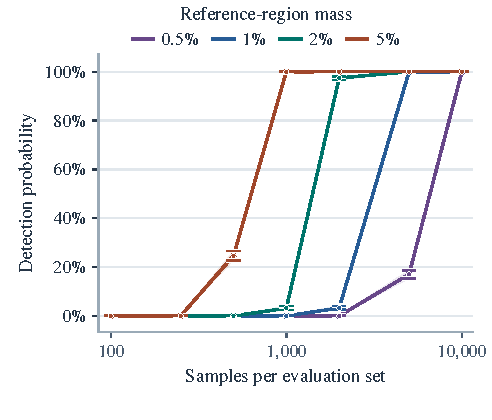
\includegraphics[width=\linewidth]{../figures/support_power_joint.pdf}
\caption{Power to certify complete region removal using the full audit's
$\alpha_{\rm occ}=0.025$, $M=10$, $\rho=0.5$, and eligibility 0.001.
Each point uses 2,000 frozen trials; whiskers and shading show exact 95\%
binomial intervals. Samples per evaluation set are shown on a logarithmic axis.}
\label{fig:support-power}
\end{figure}

\begin{table}[t]
\centering\small
\begin{tabular}{rrr rrrr}
\toprule
Mass & $n$ & & $M=10$ &40&100&440\\
\midrule
1\% &2000&&3.25&0.10&0&0\\
1\% &5000&&99.90&98.90&95.20&73.95\\
2\% &2000&&97.40&80.75&58.75&23.55\\
0.5\% &10000&&99.95&98.60&94.85&72.80\\
\bottomrule
\end{tabular}
\caption{Complete-removal detection probability (\%) as the declared family
grows, reusing the same raw counts. All entries use occupancy error 0.025,
retention 0.5, minimum mass 0.001, and 2,000 trials.}
\label{tab:support-multiplicity}
\end{table}

For a 1\% removed region at $n=5000$, the matched-allocation power is
1998/2000 or 99.9\%; at $n=2000$ it is only 65/2000 or 3.25\%.
For a 2\% region, $n=2000$ gives 1948/2000 or 97.4\%.
The full secondary grid varies retention over $\{0.3,0.5,0.7\}$ and family size
over $\{10,40,100,440\}$, retaining all 2,016 cells.
At the original categorical-only allocation 0.05, exact binomial bounds and
additive Hoeffding bounds use the same four-endpoint Bonferroni construction.
For a 2\% removed region and $n=2000$, exact bounds detect 1981/2000 trials and
Hoeffding detects 0/2000. Both guarantee at least the same nominal family
coverage; their realized conservatism differs. Across the original 336,000
categorical trials, joint interval noncoverage is 3.823\% and one trial falsely
certifies a region whose true retention is at least 0.5. These heterogeneous
pooled rates are descriptive, not substitutes for a per-family guarantee.

Equation~\ref{eq:zerocount} also gives a practical planning limit. Even knowing
a reference mass of 0.1 exactly, observing zero candidate hits needs at least
144 candidate draws for $M=10$, occupancy error 0.025, and retention 0.5.
For 128 prompts, 29 configurations, two representations, three references, and
ten regions, the declared family would require 340 draws per prompt for this
certificate; at 1\% mass it would require 3,470. These are requirements of the specified
conservative certificate, not information-theoretic lower bounds. Eight or
16 seeds per prompt cannot establish rare-region retention under this design.
The T2I policy therefore treats prompt-level point diagnostics as routing
heuristics and validates its population outcomes on independent seeds; it
does not claim prompt-specific deletion absence.

\subsection{Comparison with NDB's regional proportion test}
NDB\cite{richardson2018ndb} compares bin proportions using a pooled two-sided
normal test and reports the fraction of statistically different bins, NDB/$K$.
We prospectively specify a secondary reanalysis of all 336,000 categorical
trials and all 7,200 Gaussian/CIFAR controls. The official implementation is
pinned to commit \texttt{a6bcb4e91198} (full hash in the source manifest); all
3,360,000 categorical per-bin decisions match it exactly. To isolate the
statistical rule, every method receives identical fixed regions and independent
reference/generated evaluation counts. This is an adaptation of NDB's test,
not a comparison with its original pixel representation and training-count fit.
We retain its published per-bin significance 0.05 and add a separate
Bonferroni variant with per-bin significance $0.025/K$.

\begin{table}[t]
\centering\small
\begin{tabular}{rrrrr}
\toprule
$q/p$ & $n$ & NDB & NDB adjusted & Certificate\\
\midrule
1 &1000&4.80&0.10&0\\
0 &1000&99.30&51.55&0\\
0 &2000&100&99.55&3.25\\
0 &5000&100&100&99.90\\
0.5 &5000&83.40&44.55&0\\
\bottomrule
\end{tabular}
\caption{Target-region rejection/certification rates (\%) for reference mass
1\%, ten bins, and 2,000 frozen trials per row. NDB tests equality $q=p$;
the retention certificate establishes $q/p<0.5$. They answer different
questions, so these values do not measure superiority under a common null.}
\label{tab:support-ndb}
\end{table}

Table~\ref{tab:support-ndb} shows NDB's greater sensitivity to smaller changes.
At true retention 0.5, its equality rejection is a correct finding, while a
strictly-below-0.5 certificate should remain unresolved. Under the identical
ten-bin null with a 1\% target and $n=1000$, original mean NDB/$K$ is 0.05215;
the probability of any flagged bin is 40.65\%. The adjusted variant's any-bin
rate is 2.45\%. Original NDB's per-bin level is not a familywise guarantee.
Both NDB variants detect every Gaussian quadrant-removal trial; for the CIFAR
region removal at $n=1000$, both detect 200/200 versus 196/200 retention
certificates. Thus clustering-based loss detection is established prior work;
the audit adds an explicit effect-size resolution and combines its output with
spread, fidelity, and intervention validation. All counts, normalized scores,
Jensen--Shannon divergences, null rates, and trial-proportion intervals appear
in \texttt{ndb\_comparison.json} and its raw arrays. The adjusted normal test
remains approximate, unlike the exact binomial certificate.

\subsection{Representation and partition resolution}
As a secondary robustness analysis, we freeze the complete grid of DINO PCA
dimensions $\{16,32,64\}$ and region counts $K\in\{5,10,20\}$ for five completed
CIFAR configurations. All use the original independent 5,000/5,000/10,000
reference split, 10,000 generated images, seed 1729, and unchanged margins.
The exact occupancy family contains $3(5+10+20)5=525$ regions at
$\alpha_{\rm occ}=0.025$; the support family contains 45 comparisons at
$\alpha_{\rm support}=0.025$. Approximate spread intervals separately use
$0.05/525$. Every configuration has a contraction flag in all nine settings,
no expansion flag, and a passing feature-support gate. Leading DDIM4, Bures4,
fresh leading DDIM2, and covariance-only initialization2 have regional
depletion in all nine settings. UniPC4 has a depletion certificate in seven;
the two exceptions use five regions with 32 or 64 directions. Thus substantial
deficits persist across resolutions, while milder regional findings depend on
the partition. Default-resolution counts and tail rates exactly reproduce the
primary audit, and spread points agree within $7\times10^{-16}$; the revised
family allocation changes no default qualitative flag. All 45 results and
ineligible cells are retained; no primary choice is changed.

\begin{figure*}[t]
\centering
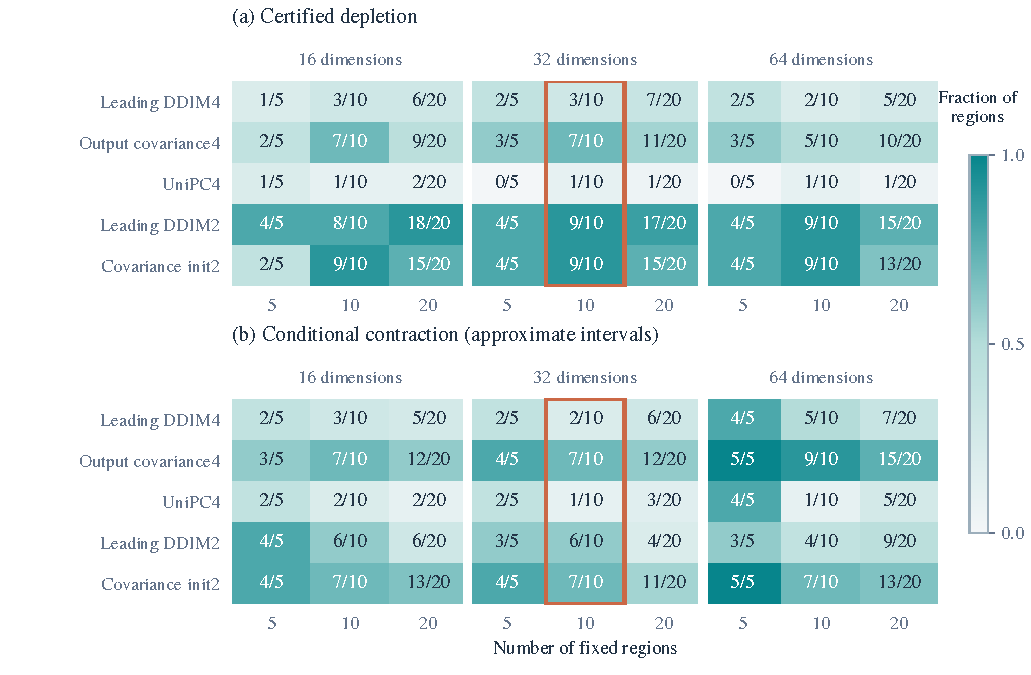
\includegraphics[width=\textwidth]{../figures/support_cifar_resolution.pdf}
\caption{Complete secondary resolution analysis. Entries count flagged regions
out of all $K$ fixed regions; red outlines mark the default 32-direction,
ten-region representation. A region without a spread flag can be unresolved
or have fewer than 30 samples. All 45 support gates pass and no expansion flag
occurs, so the figure displays the two varying outputs. Region identities
change with the resolution; fractions of regions are not fractions of data
probability. Full counts, intervals, eligibility and source hashes accompany
the results.}
\label{fig:support-resolution}
\end{figure*}

\subsection{Interpretation and executable outputs}
The output contains the fixed reference, feature representation, regions,
calibration thresholds, sample counts, ratio intervals, eligibility, unresolved
tests, supported deficit flags, and recommended next comparison. A support
departure is called off-reference expansion only if expansion is independently
supported. The training-comparison branch requires a data reference,
independently validated semantic measurements, a certified data-relative
imbalance (depletion or excess), acceptable resolved-model fidelity, and persistence under
alternative resolved samplers. Otherwise the next step is a controlled sampler
comparison or additional measurement. Invertible contraction can move probability
across a fixed feature boundary; therefore even certified regional depletion
cannot identify a missing semantic mode or unique historical cause.

The practitioner entry point \texttt{audit\_features.py} accepts separate
NPZ fit, calibration, reference-evaluation and candidate arrays, named feature
and sample-ID keys, and a complete frozen configuration. It checks finite
dimensions and declared sample-ID disjointness, records input hashes, and emits
strict JSON measurements and interpretation. External fidelity remains
unmeasured unless supplied explicitly with its evidence source. The delivered
CIFAR example reproduces the original regional intervals and support gate;
synthetic interface checks reject overlapping IDs and invalid evidence.

The complete controlled validation takes 276 seconds on CPU with one BLAS
thread and no GPU. Run \texttt{support\_validate.py --run}, followed by
the supplied secondary-analysis and plotting scripts. These scripts preserve
the frozen raw trials, record source and output hashes, and regenerate editable
vector figures. External fidelity and learned-model intervention outcomes
are reported in their respective experiments rather than inferred from these
feature controls.

\subsection{Two-sided mass balance with shared reference uncertainty}
\label{sec:support-mass-balance}
Severe relative depletion and useful mass balance ask different questions.
For a fixed semantic region, let $p_j$ and $q_{aj}$ be its probabilities under
data and candidate~$a$, respectively, using all images as the denominator.
A candidate can retain a class while allocating too much probability to it.
We therefore also use a prespecified absolute balance tolerance~$\delta$.
This complements the relative-depletion test: a region of mass at most
$\delta$ can disappear without violating an absolute tolerance.

Suppose the study declares $R$ distinct reference-region intervals and $C$
candidate-region intervals. Allocate fraction $w$ of total error $\alpha$ to
the reference. The Clopper--Pearson intervals~\cite{clopper1934confidence}
$[p_j^-,p_j^+]$ have each tail $\alpha w/(2R)$, and
$[q_{aj}^-,q_{aj}^+]$ have each tail $\alpha(1-w)/(2C)$.
A union bound gives simultaneous coverage at least $1-\alpha$ for all
declared masses. On that event,
\begin{equation}
q_{aj}-p_j\in I_{aj}
=[q_{aj}^- -p_j^+,\ q_{aj}^+-p_j^-].
\label{eq:supp_shared_mass_difference}
\end{equation}
Charging each shared reference interval once avoids a redundant multiplicity
penalty. Independence between candidates or between regions is unnecessary;
independent evaluation rows within each fixed population remain required.
This guarantee conditions on the trained models and fixed measurement functions.

We certify excess if $\inf I_{aj}>\delta$, depletion if
$\sup I_{aj}<-\delta$, and equivalence if
$I_{aj}\subseteq[-\delta,\delta]$; all remaining cases are inconclusive.
All-class equivalence requires every interval to be contained. Persistent
imbalance requires the same class and direction under all declared resolved
samplers, with every sampler fidelity-qualified. Certified balance requires
all-class equivalence and fidelity qualification under every probe. Mixed
directions are retained; inconclusive outcomes do not imply a numerical-only
cause. These are operational statements, not identification of a unique cause.
When data representativeness is an objective and validated data regions are
available, the data audit is performed regardless of teacher-relative flags.
A teacher and all its samplers can share the same imbalance; agreement with
the teacher alone cannot establish data-relative balance.

The separately frozen MNIST balance follow-up uses $\alpha=.025$, $w=1/2$,
$R=10$, $C=360$, and $\delta=.03$, with complete $.02/.04$ sensitivity.
The margin is three percentage points of unconditional mass, approximately
30\% of a nominal balanced digit class; it is domain-specific. All 10,000 real
test images are available for semantic counts because classifiers and their
threshold were fixed using training data. Geometry retains its independent
fit/calibration/evaluation pools. Rejection remains a separate fidelity event.

Sample size was chosen before fresh follow-up training from 20,000 synthetic
multinomial trials per setting, using the old reference proportions. With
16,000 generated and 10,000 reference images, excess at $q_3=.16$ versus
$p_3=.0983$ is certified in 99.23\% of trials
(95\% Monte Carlo interval: 99.10--99.35\%); reference-matched masses yield
all-class equivalence in 95.58\% (95.29--95.86\%). With $q_3=.087$, all-class
equivalence remains only 45.12\% (44.42--45.81\%). Thus the design permits
meaningful inconclusive outcomes rather than relaxing the tolerance to obtain
a pass. Complete grids include 5,000/10,000 reference images and
8,000/16,000/32,000/64,000 generated images.

The reusable \texttt{diagnostic\_mass\_balance.py} API and counts-JSON CLI
implement these rules. The study wrapper verifies all 36 diagnosis artifacts
and freezes every label before independent outcome generation. The original
relative-depletion API and its recorded results remain unchanged. Paired
fidelity and separate support families receive errors $.0125$ each, so their
union with the mass family is bounded by $.05$. Full-data self-comparisons are
explicit structural identity anchors, not evidence of absolute visual fidelity.
The joint statement averages over the sampled real-reference pools, conditional
on the trained generators and frozen classifiers. Semantic bounds use all
10,000 reference rows and are not additionally conditioned on the realized
geometry-fit subset. Geometry-based bounds condition on their independent
fitting pools and then average over them; the union bound does not require
independence between these families.
